\begin{section_2}
\subsection{Код}
\begin{lstlisting}[language=Python]
import numpy as np
import matplotlib.pyplot as plt
import matplotlib.colors as clr
from itertools import cycle
import os

def mandelbrot(pmin, pmax, qmin, qmax, ppoints=1000, qpoints=1000,
              max_iterations=300, infinity_border=10):
   image = np.zeros((ppoints, qpoints))
   p, q = np.mgrid[pmin:pmax:(ppoints*1j), qmin:qmax:(qpoints*1j)]
   c = p + 1j*q
   z = np.zeros_like(c)
   for k in range(max_iterations):
       z = z**2 + c
       mask = (np.abs(z) > infinity_border) & (image == 0)
       image[mask] = k
       z[mask] = np.nan
   return -image.T

def make_colormap():
   colorpoints = [
       (1 - (1 - q)**4, c)
       for q, c in zip(
           np.linspace(0, 1, 20),
           cycle(['#ffff88', '#000000', '#ffaa00'])
       )
   ]
   return clr.LinearSegmentedColormap.from_list('mycmap', colorpoints, N=2048)

def render(image, bounds, cmap, filename):
   """Отрисовка и сохранение фрактала"""
   pmin, pmax, qmin, qmax = bounds
   fig, ax = plt.subplots(figsize=(8, 8))
   ax.imshow(image, extent=(pmin, pmax, qmin, qmax), cmap=cmap, interpolation='none')
   ax.set_title(f"Множество Мандельброта\nRe∈[{pmin:.2f},{pmax:.2f}] Im∈[{qmin:.2f},{qmax:.2f}]",
                color='white', fontsize=10)
   ax.set_xticks([]); ax.set_yticks([])
   ax.set_facecolor('black')
   plt.tight_layout()
   os.makedirs("tfkp", exist_ok=True)
   plt.savefig(os.path.join("tfkp", filename), dpi=300, bbox_inches='tight', facecolor='black')
   plt.close(fig)
   print(f"Сохранено: tfkp/{filename}")

if __name__ == "__main__":
   cmap = make_colormap()
   full_bounds = (-2.5, 1.5, -2.0, 2.0)
   image = mandelbrot(*full_bounds, 1000, 1000, max_iterations=300)
   render(image, full_bounds, cmap, "mandelbrot_full.png")
   zooms = [
       (-0.75, -0.70, 0.05, 0.10), 
       (-1.25, -1.15, 0.20, 0.30),  
       (0.25, 0.35, -0.65, -0.55),  
       (-1.40, -1.20, -0.05, 0.05),
       (0.35, 0.45, 0.35, 0.45)      
   ]

   for i, b in enumerate(zooms, start=1):
       img_zoom = mandelbrot(*b, 1500, 1500, max_iterations=800)
       render(img_zoom, b, cmap, f"mandelbrot_zoom_{i}.png")

   print("Все изображения сохранены")

\end{lstlisting}
\subsection{Картинки}
\begin{figure}
    \centering
    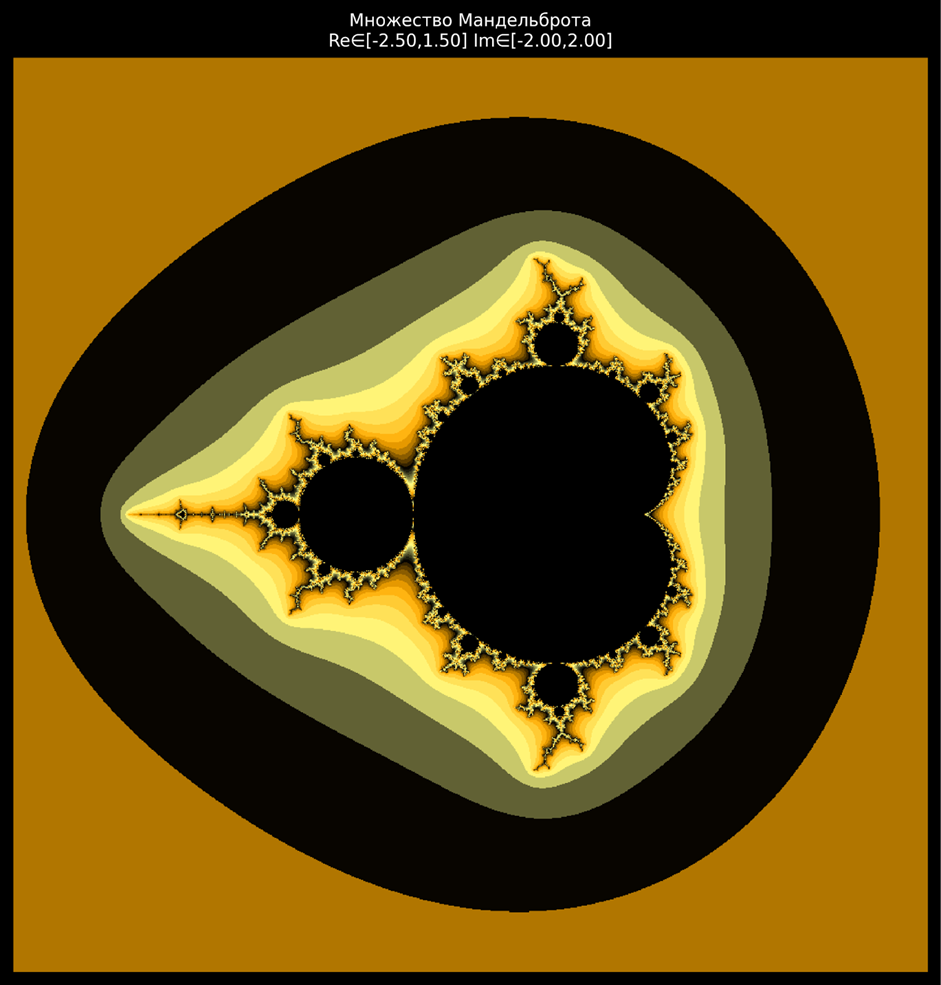
\includegraphics[width=1\linewidth]{photo/image1.png}
    \label{fig:placeholder}
\end{figure}
\begin{figure}
    \centering
    
\includegraphics[width=1\linewidth]{photo/image2.png}
    \label{fig:placeholder}
\end{figure}
\begin{figure}
    \centering
    
\includegraphics[width=1\linewidth]{photo/image3.png}
    \label{fig:placeholder}
\end{figure}
\begin{figure}
    \centering
    
\includegraphics[width=1\linewidth]{photo/image4.png}
    \label{fig:placeholder}
\end{figure}
\begin{figure}
    \centering
    
\includegraphics[width=1\linewidth]{photo/image5.png}
    \label{fig:placeholder}
\end{figure}
\end{section_2}